\documentclass{exos}
\usepackage{main}

\title{Exercices : Arbres Pondérés}
\author{Premières Spécialité Mathématiques}
\date{Chapitre 6 Partie 2}

\begin{document}
\maketitle
\begin{minipage}[t]{0.45\textwidth}
\begin{center}
\textbf{Utiliser les arbres pondérés}
\end{center}
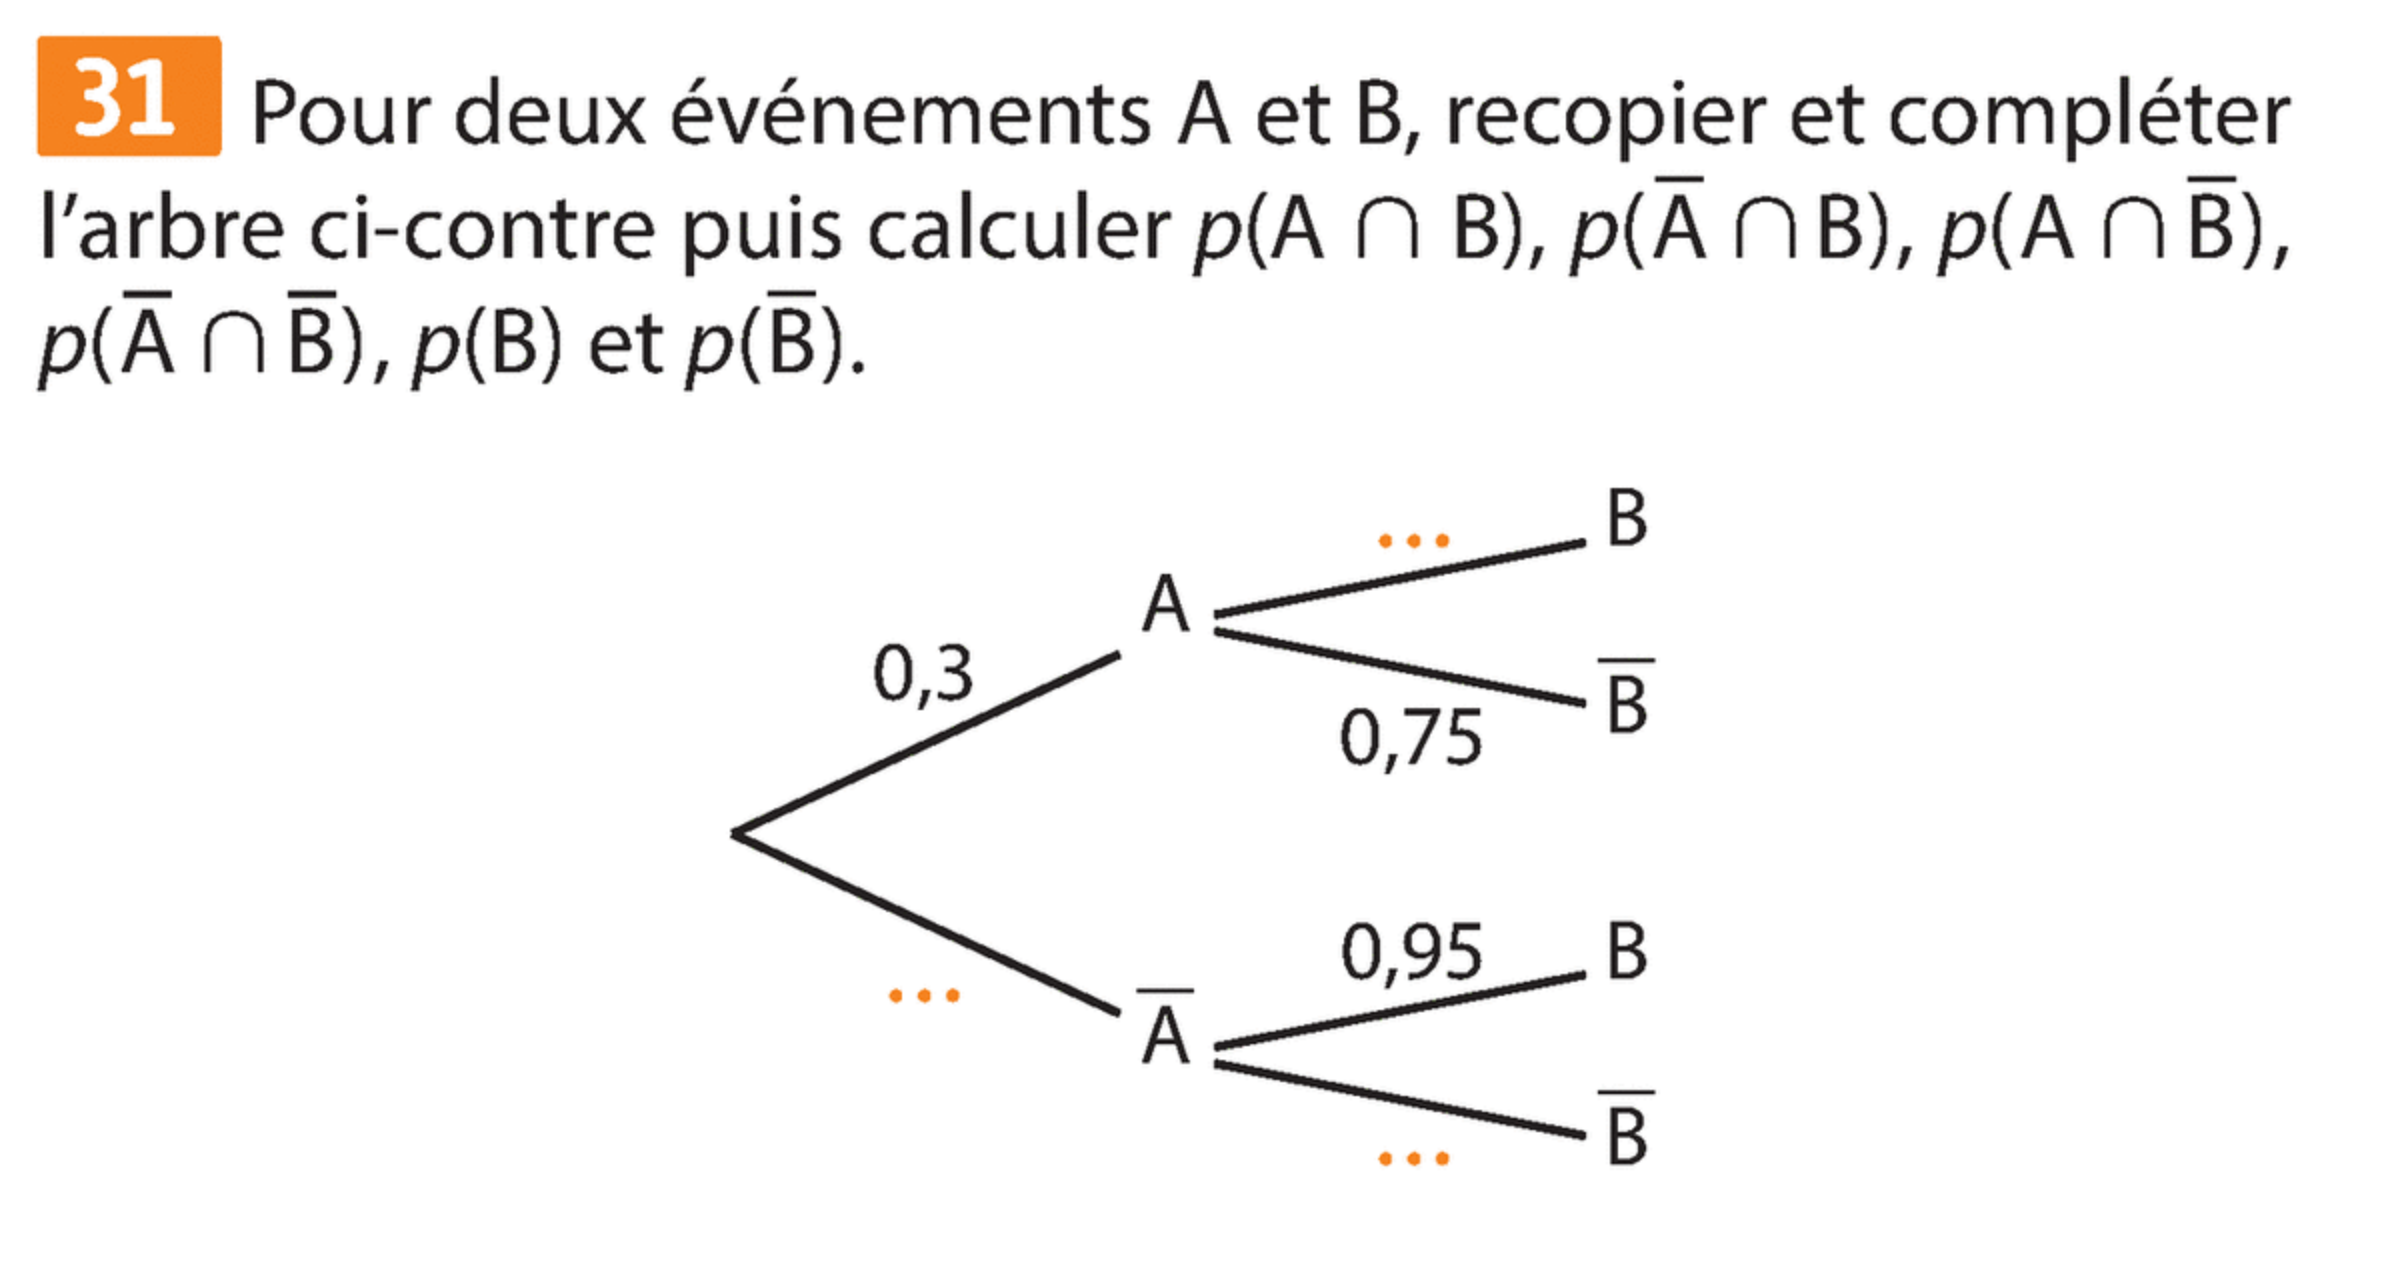
\includegraphics[width=\textwidth]{Exo_31.png}
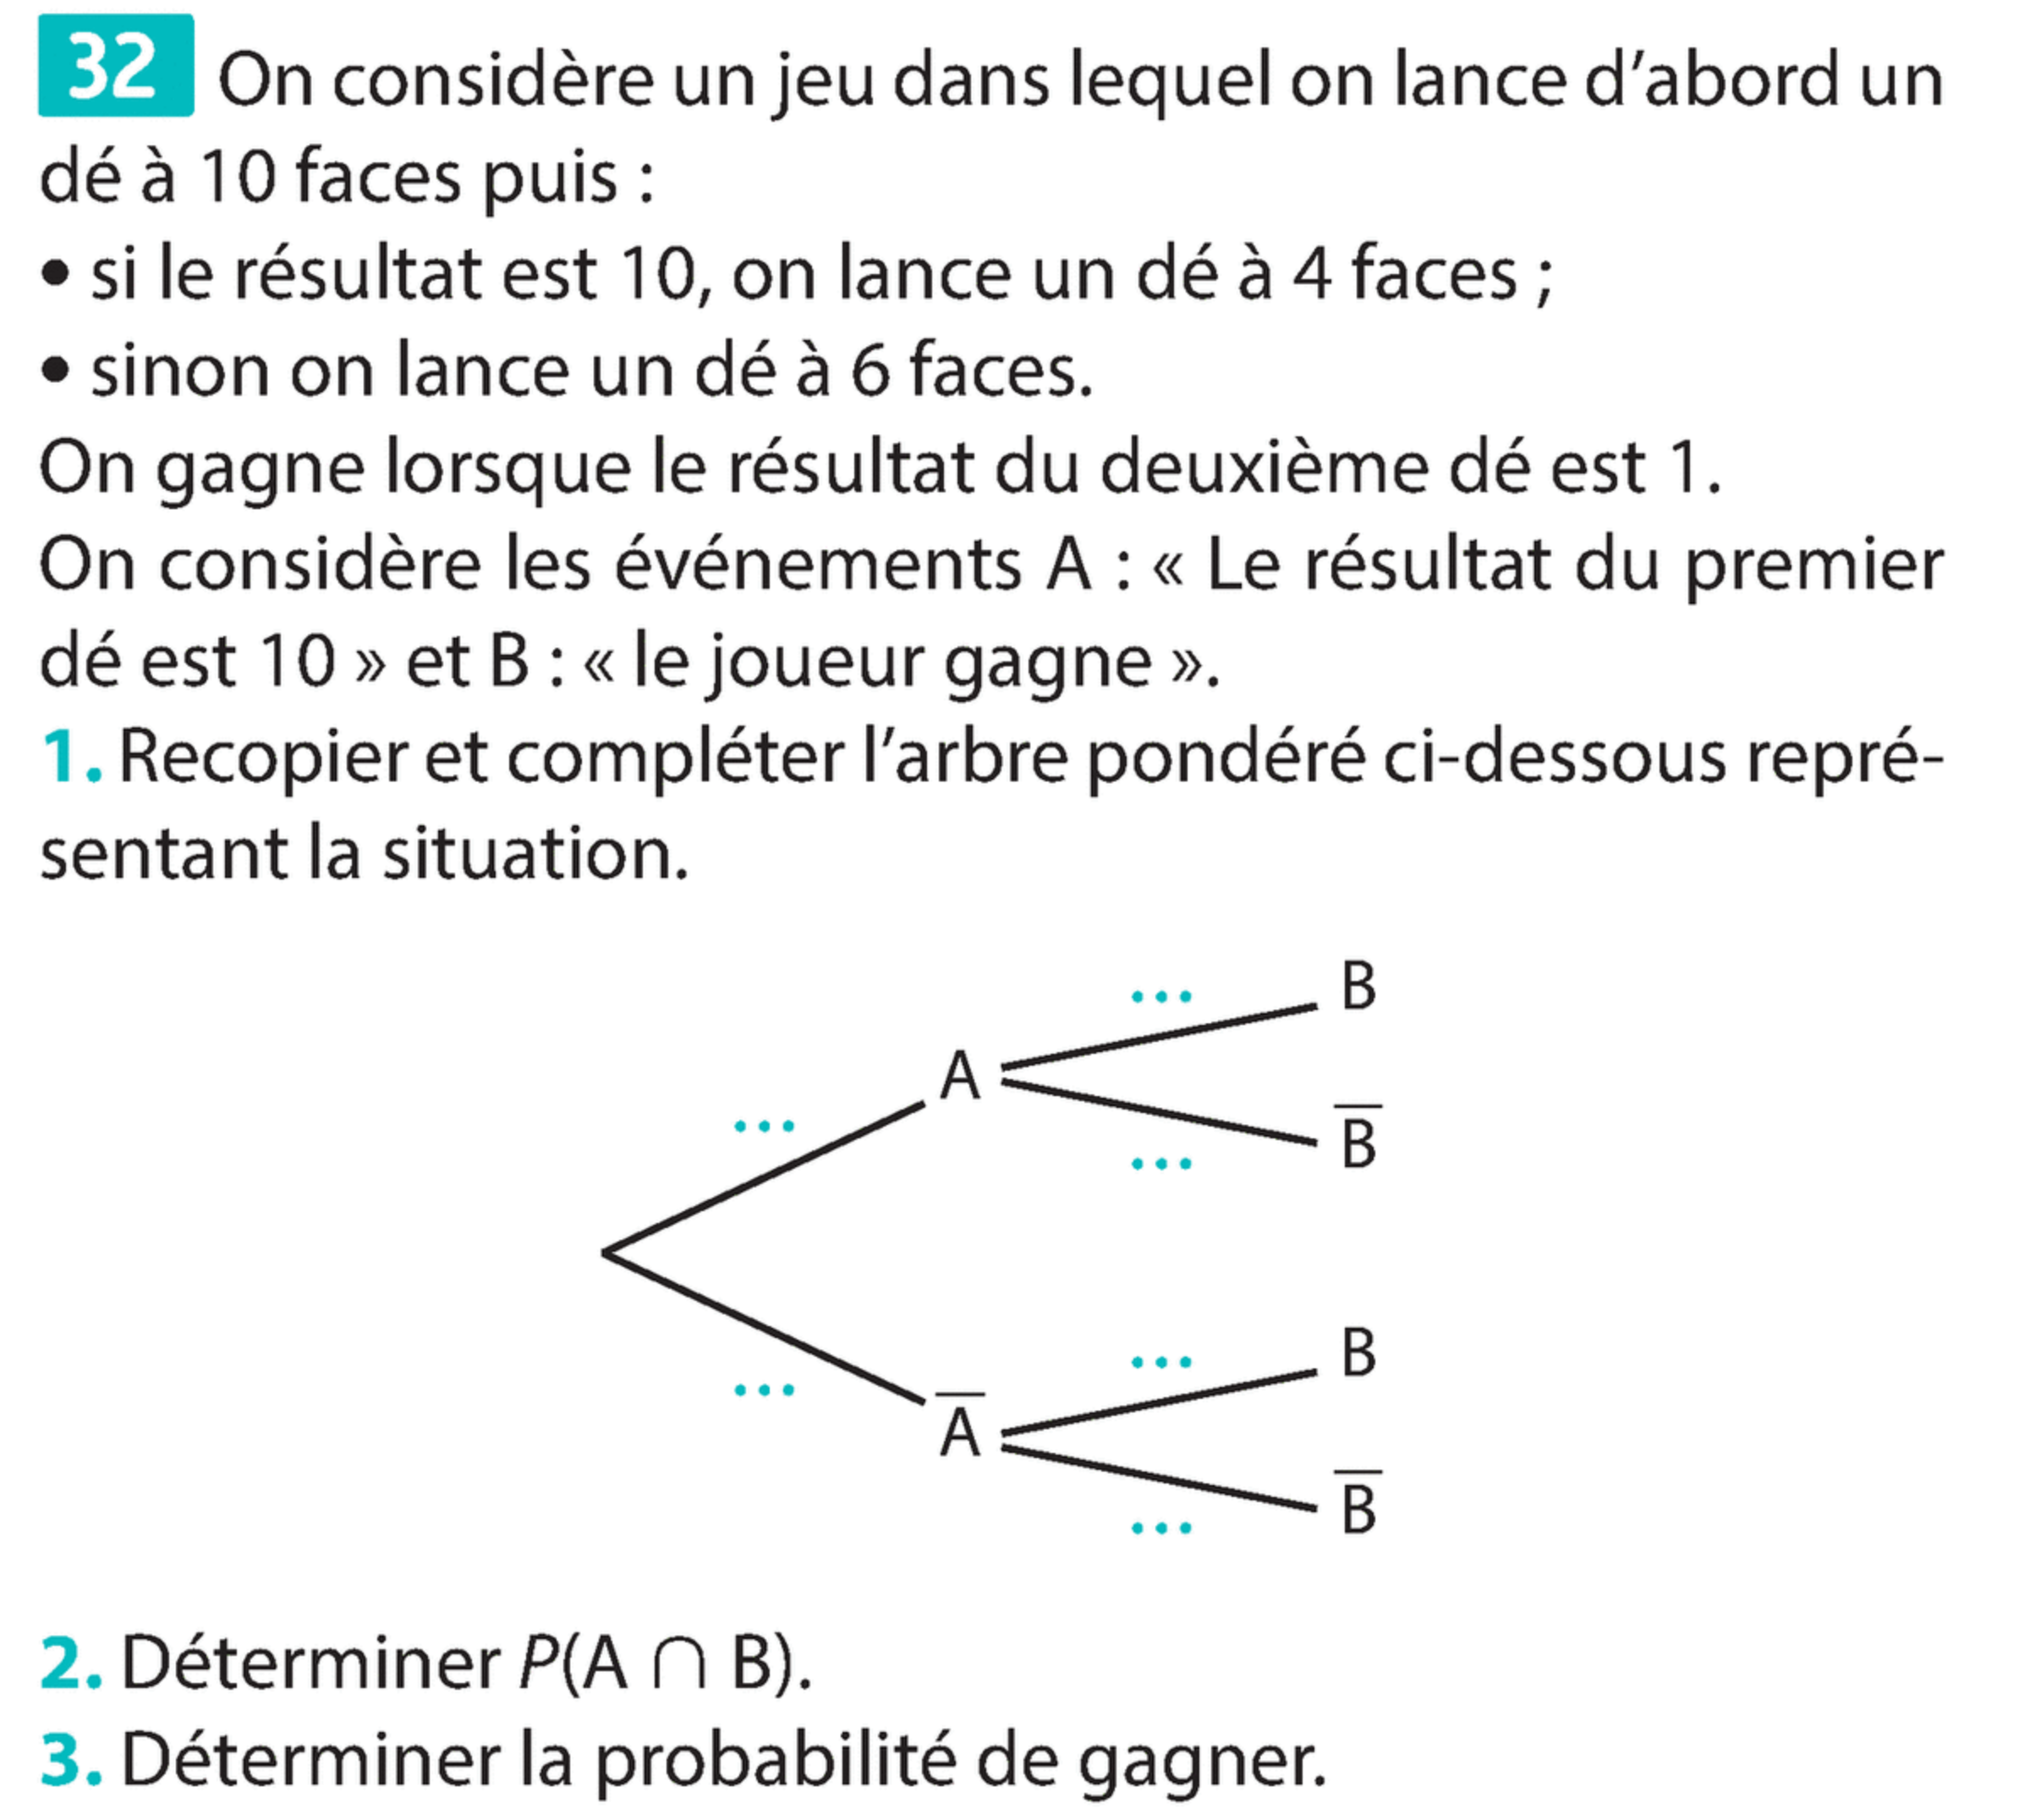
\includegraphics[width=\textwidth]{Exo_32.png}
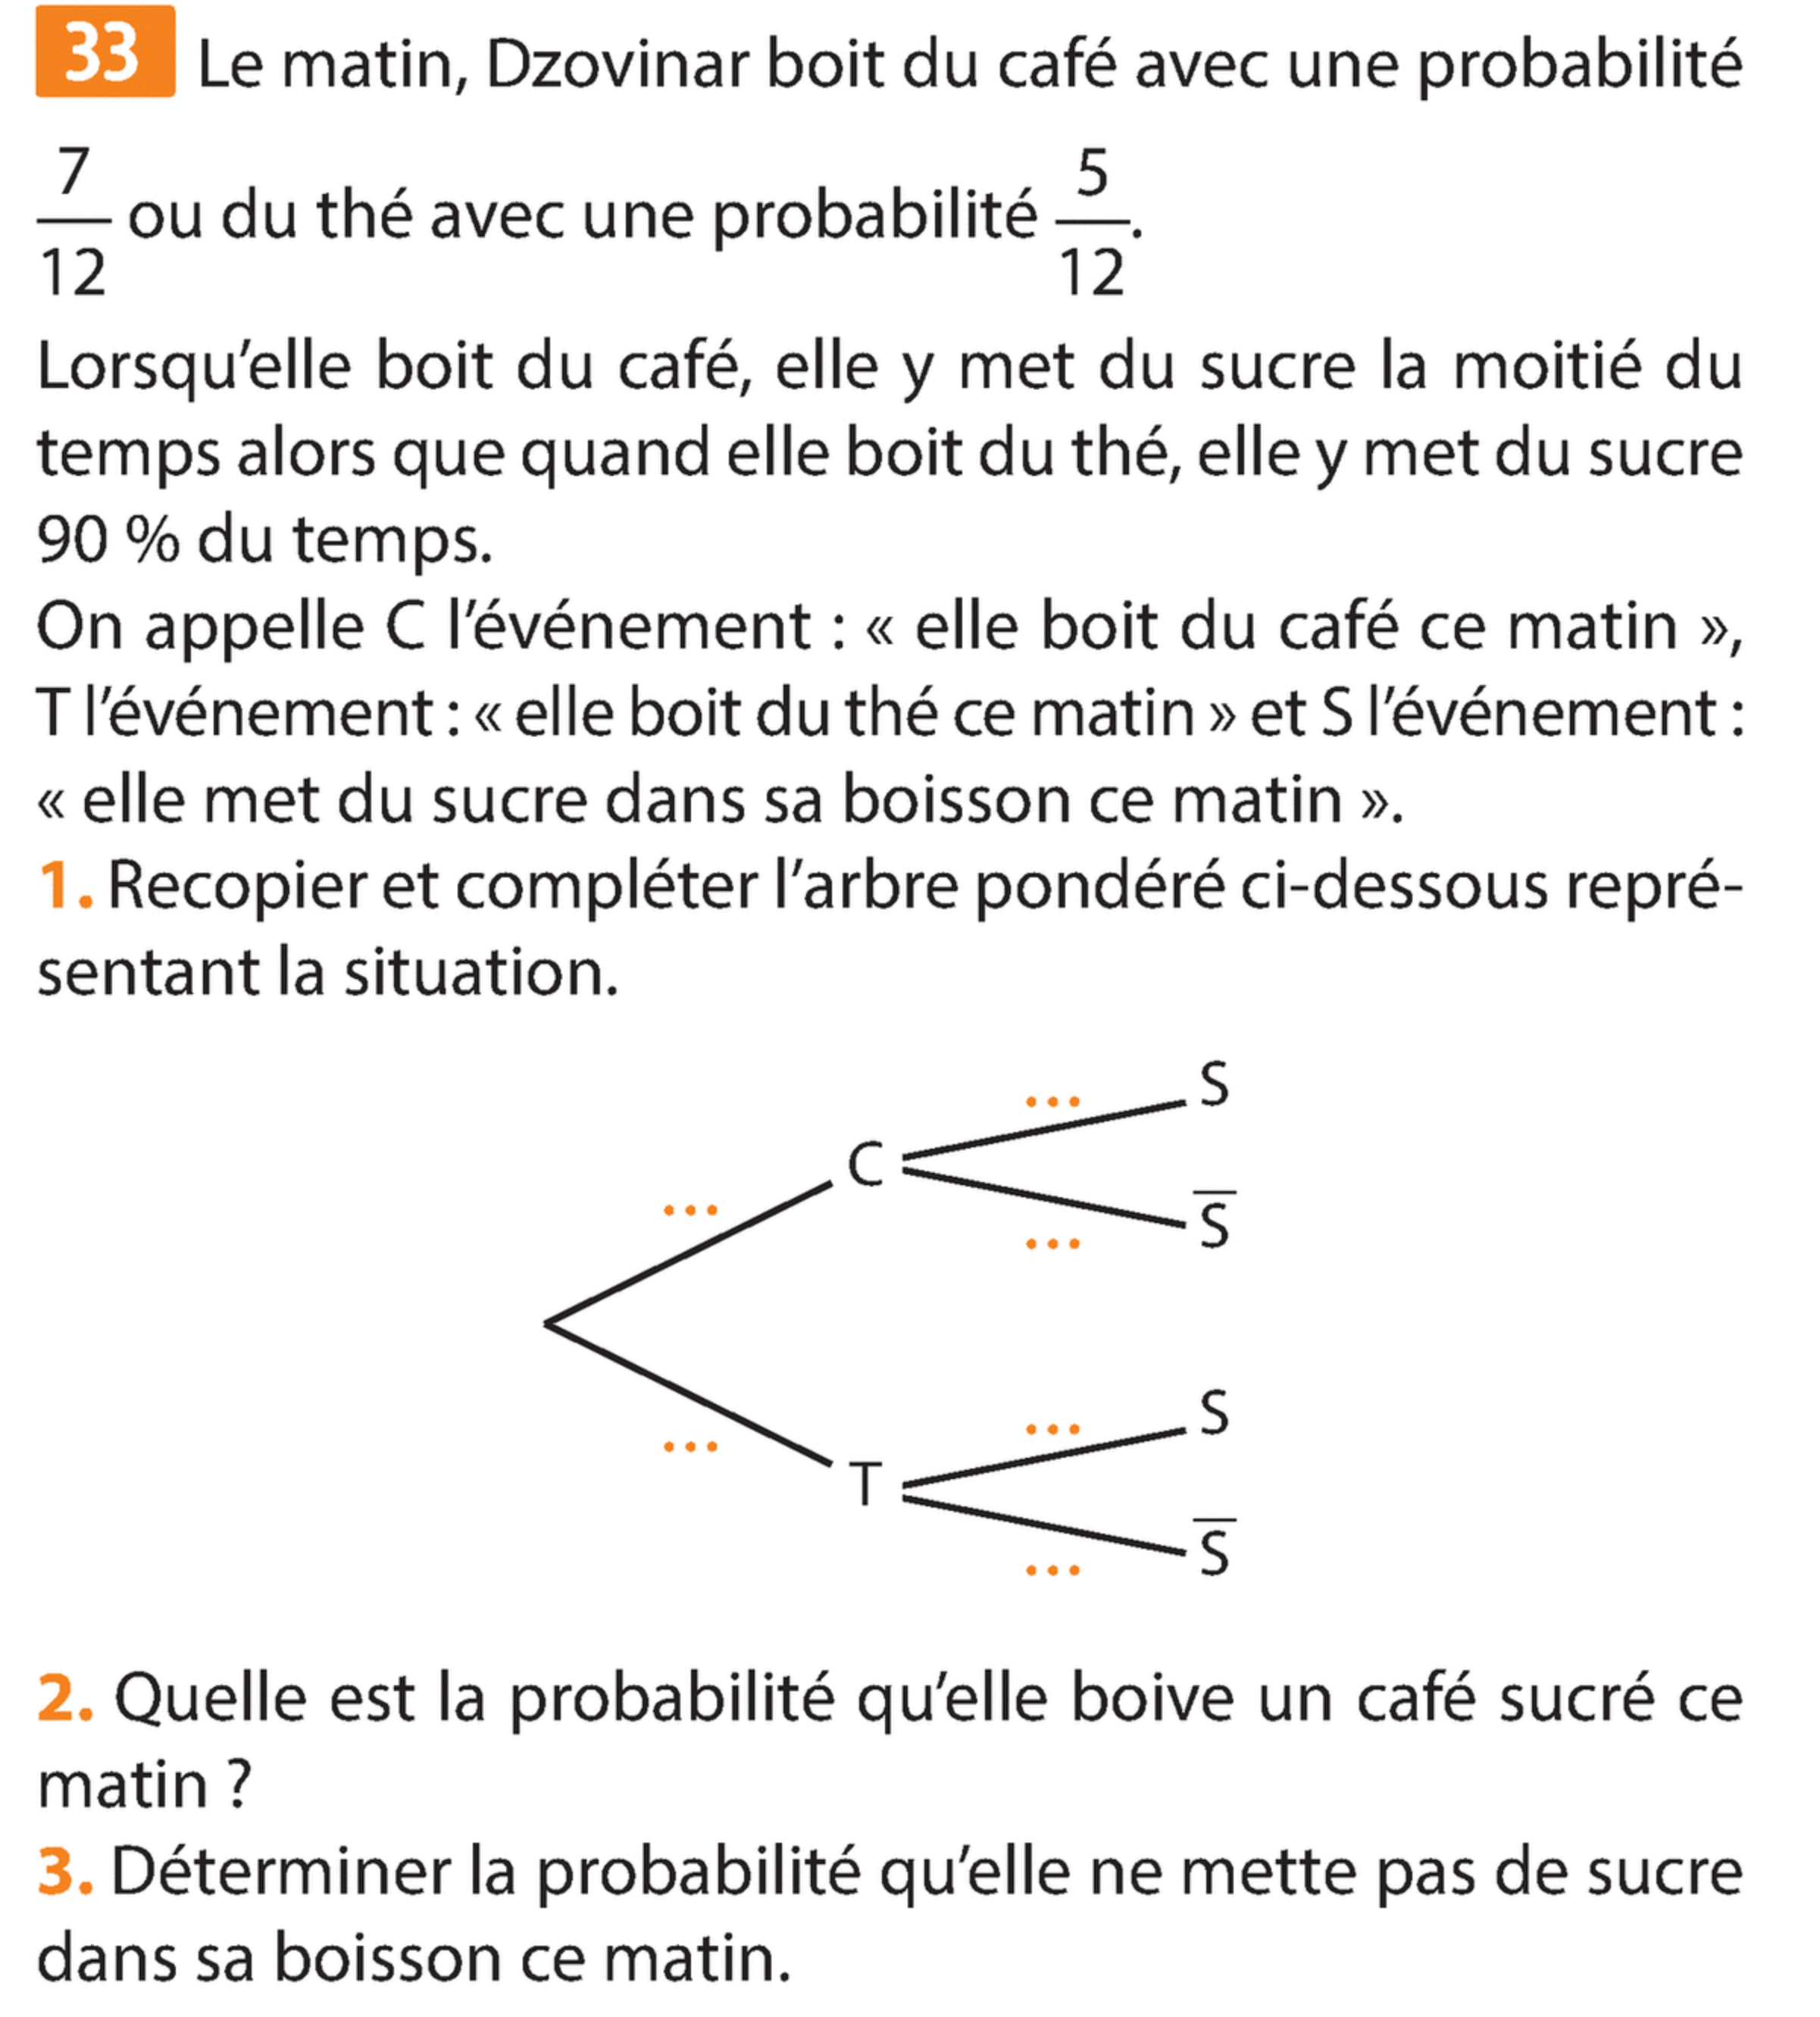
\includegraphics[width=\textwidth]{Exo_33.png}
\end{minipage}
\hfill\vline\hfill
\begin{minipage}[t]{0.45\textwidth}
\begin{center}
\textbf{Construire les arbres pondérés}
\end{center}
% 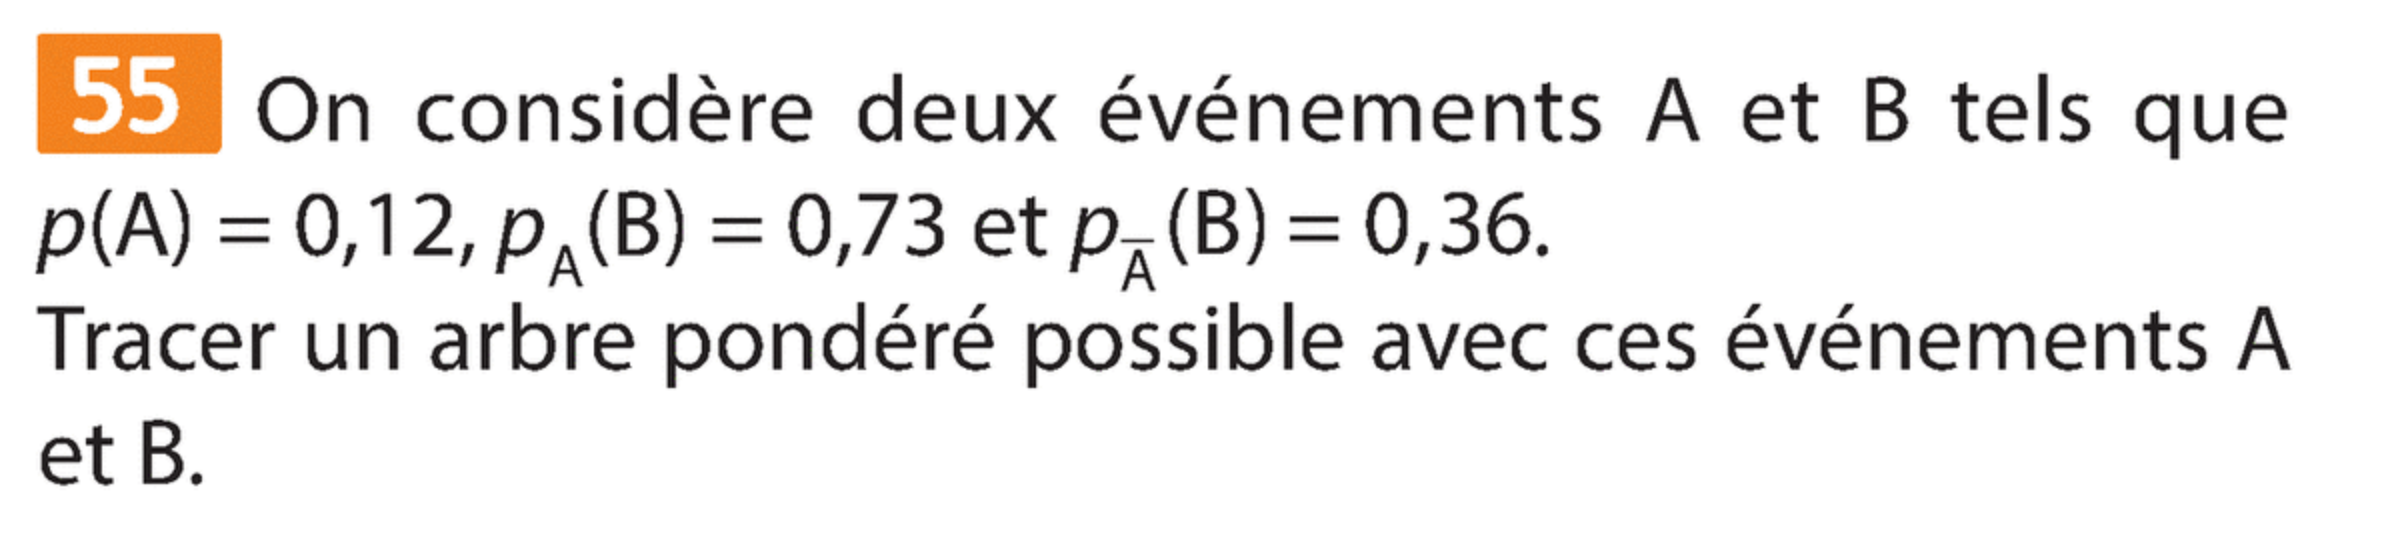
\includegraphics[width=\textwidth]{Exo_55.png}
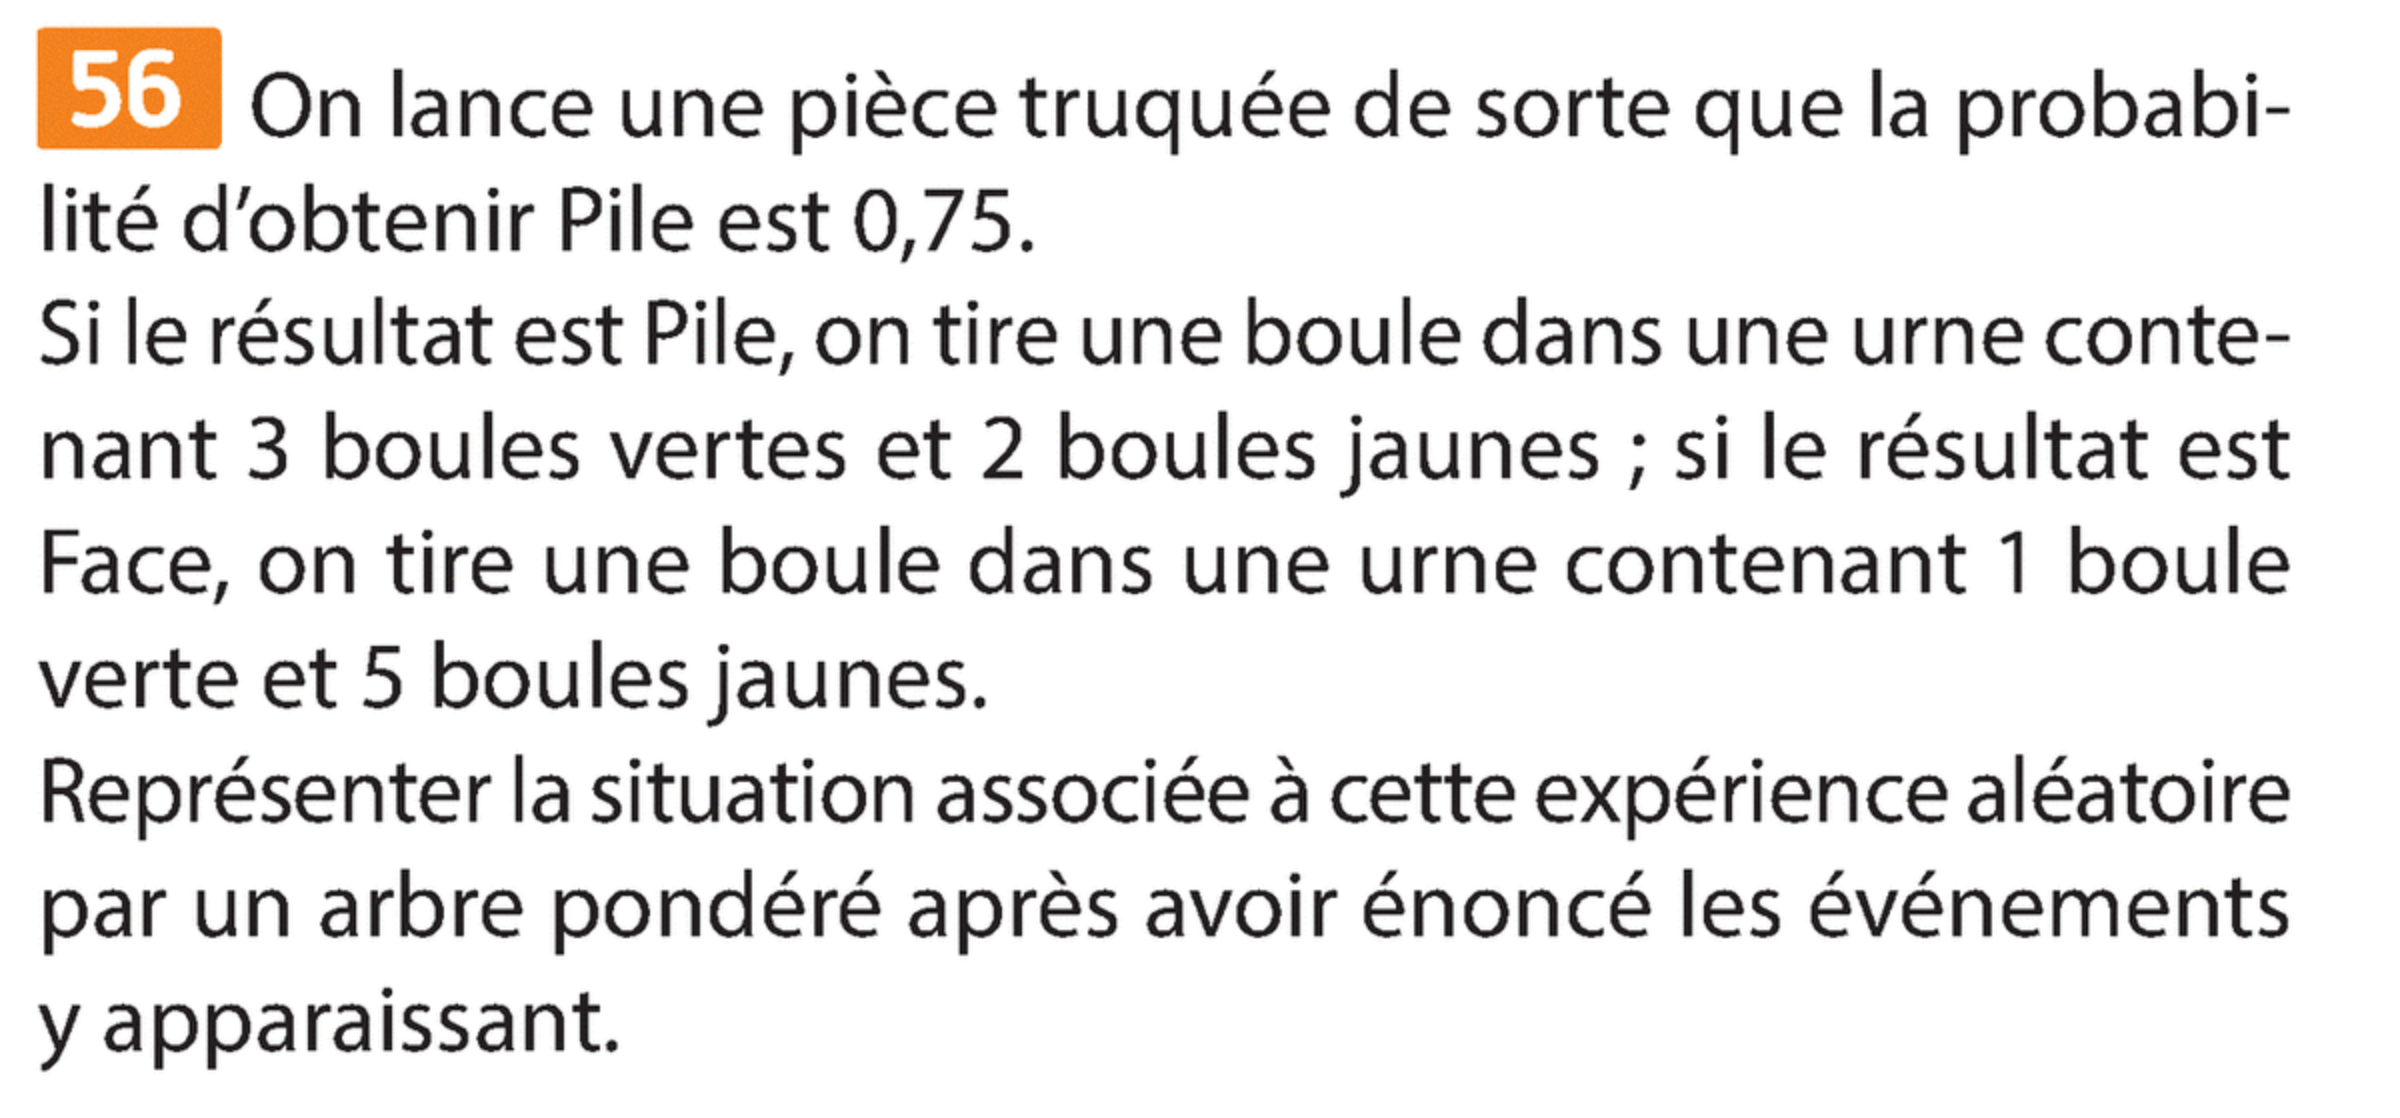
\includegraphics[width=\textwidth]{Exo_56.png}
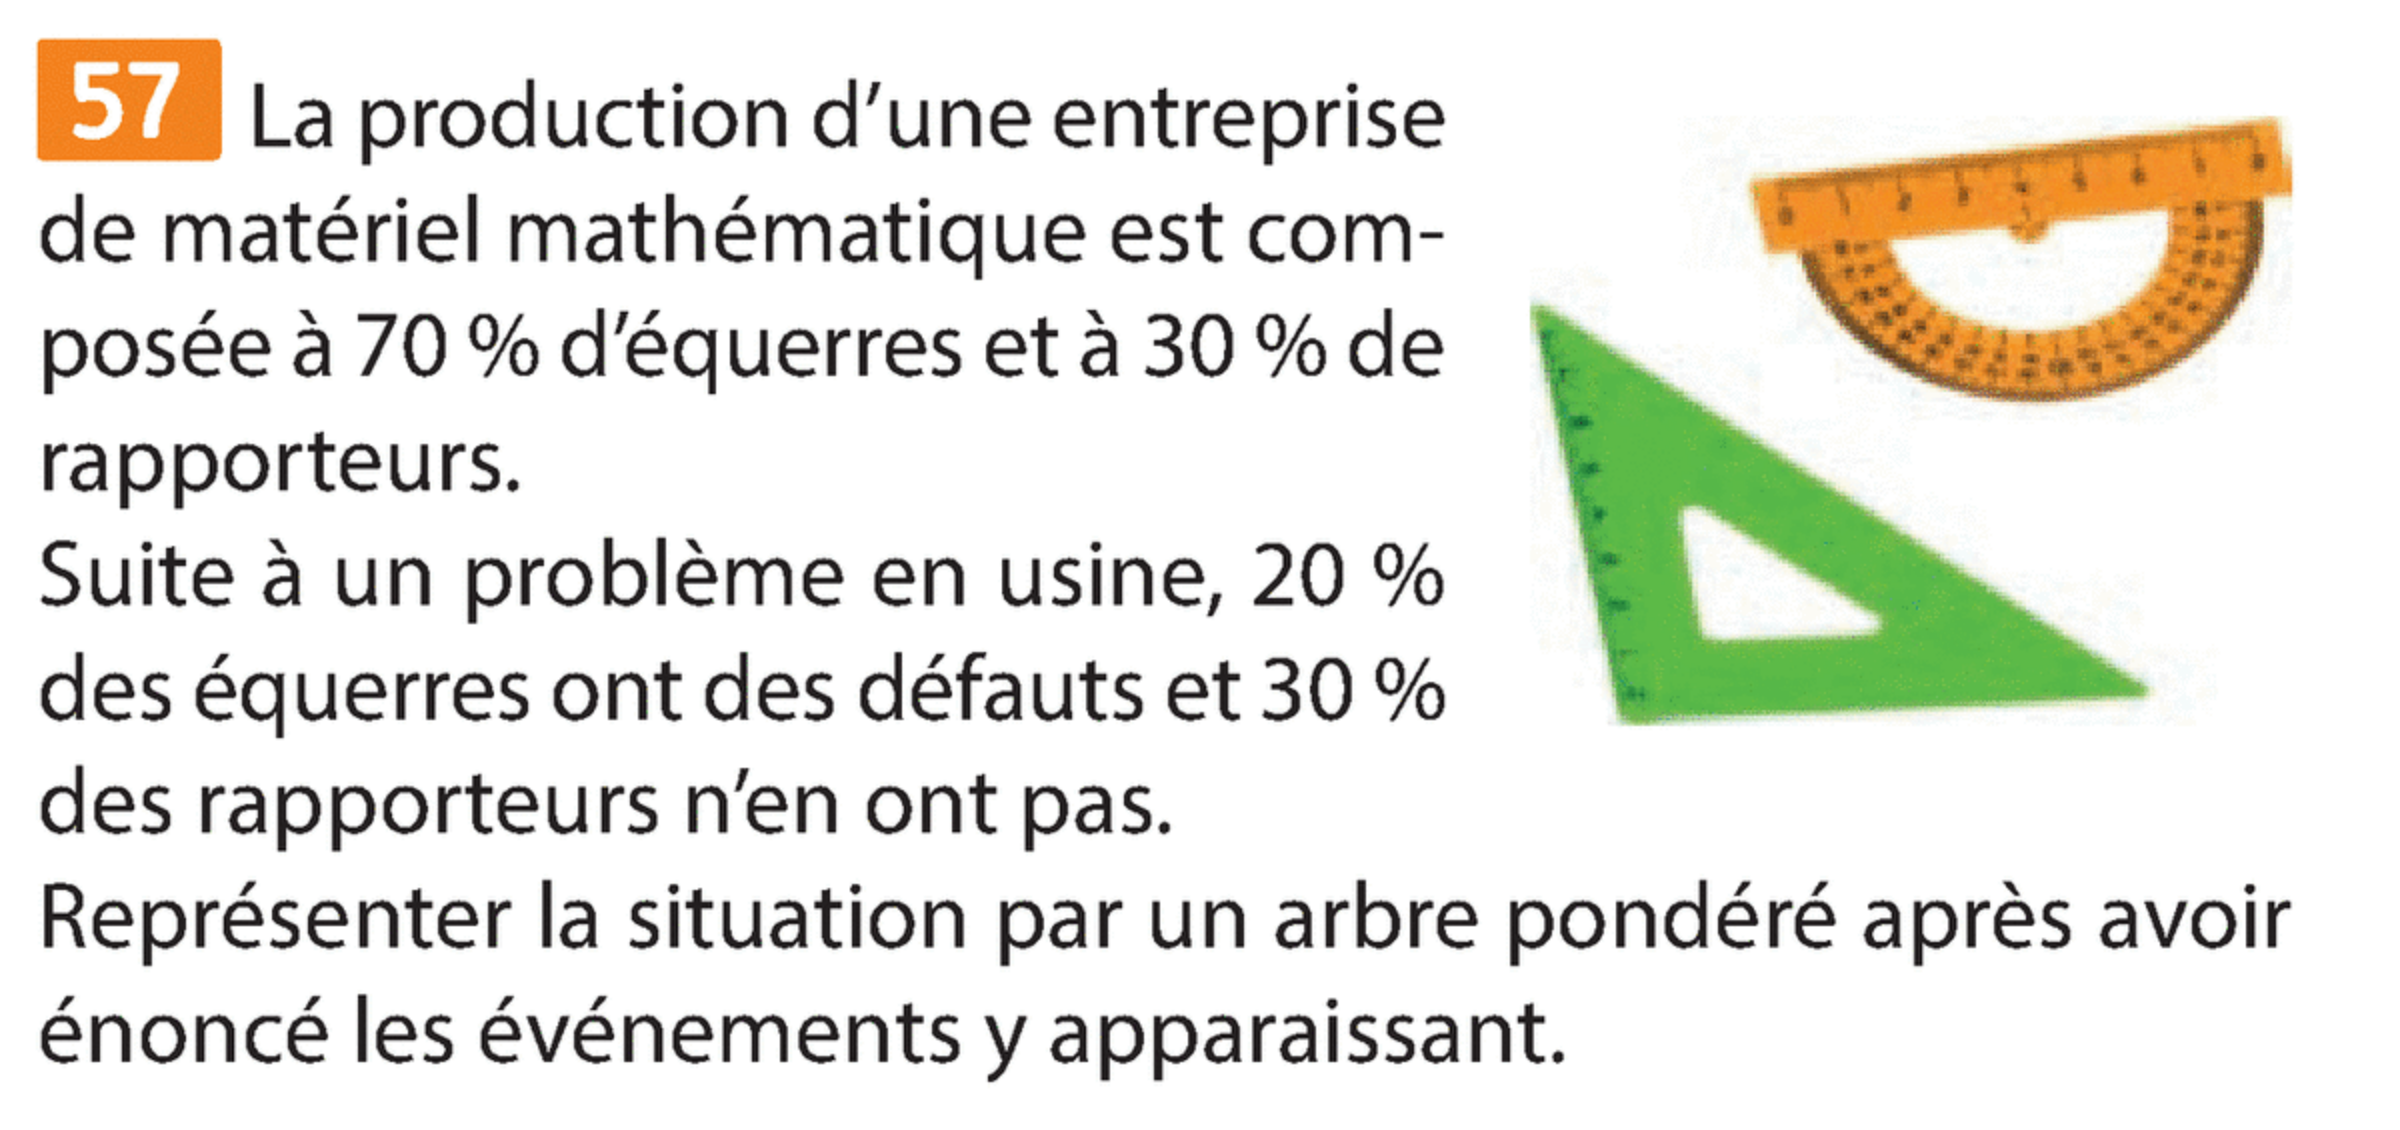
\includegraphics[width=\textwidth]{Exo_57.png}
\begin{center}
\textbf{Probabilités et suites}
\end{center}
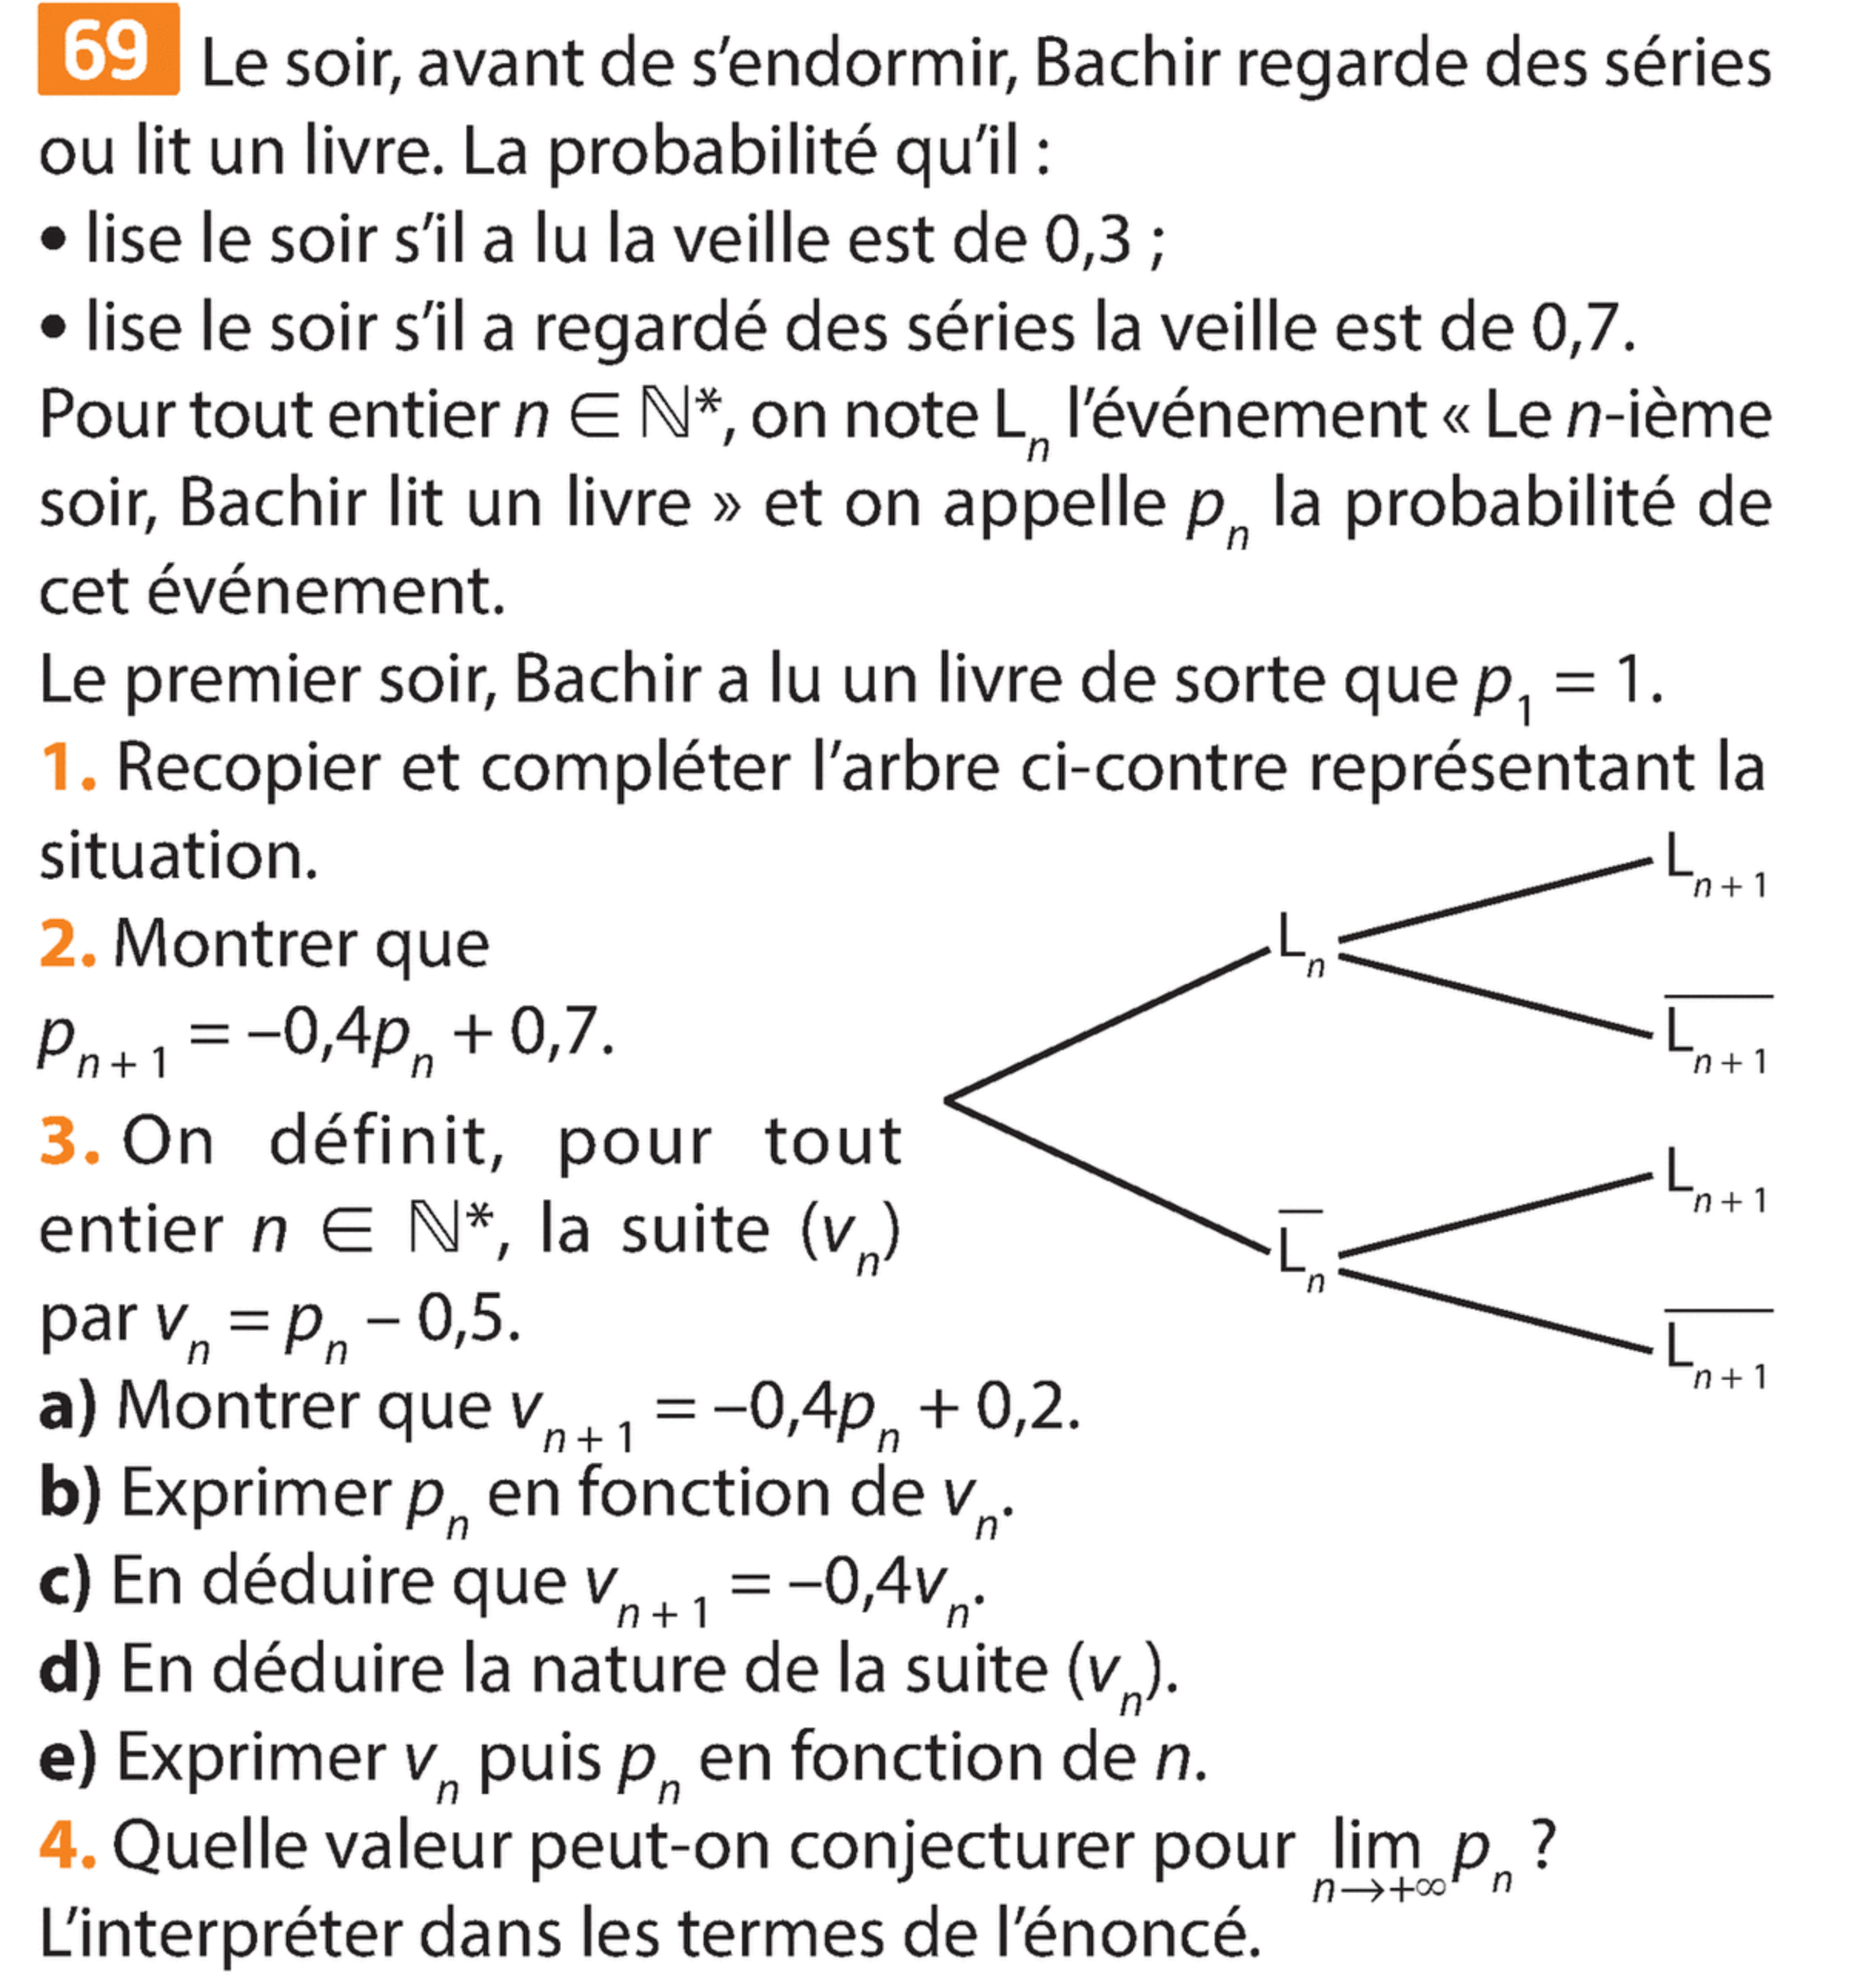
\includegraphics[width=\textwidth]{Exo_69.png}
\end{minipage}
\end{document}
